\documentclass{scrbook}
\usepackage{biblatex}
\bibliography{refs}
\usepackage{epigraph} 
\usepackage[utf8]{inputenc}
\usepackage{amsthm}
\usepackage{amsfonts}
\usepackage{amsmath}
\usepackage{float}
\usepackage{graphicx}

\graphicspath{ {./images/} }

\newtheorem{theorem}{Theorem}[section]
\newtheorem{corollary}{Corollary}[section]
\theoremstyle{definition}
\newtheorem{definition}{Definition}[section]
\newtheorem{lemma}{Lemma}
\newtheorem{conjecture}{Conjecture}
\newtheorem{proposition}{Proposition}
\newtheorem{approach}{Approach}
\newtheorem{example}{Example}

\newtheorem{exerciseinner}{Exercise}
\newenvironment{exercise}[1]{%
  \renewcommand\theexerciseinner{#1}%
  \exerciseinner
}{\endexerciseinner}

\newcommand{\R}{\mathbb{R}}
\newcommand{\N}{\mathbb{N}}
\newcommand{\Q}{\mathbb{Q}}
\newcommand{\Z}{\mathbb{Z}}

\title{A Review of Basic Algebra and Single-Variable Calculus}
\subtitle{The Indefinitive Guide}
\author{Junhyun Lim}

\begin{document}
\maketitle

\tableofcontents

\chapter*{Preface}
\addcontentsline{toc}{chapter}{Preface}

This is a series of lecture notes to-be-updated continuously for you, the reader. As the text assumes some knowledge of algebra and calculus, it will instead focus more so on review of the material and in-depth approach to their concepts. 

The book may skip several topics deemed unimportant to review depending on your knowledge and background as an accounting major. However, if you wish to learn more about a given topic, feel free to ask. A section will be added when appropriate and you will be shortly notified once completed. 

As this is the first time I'm writing a lengthy piece of educational purposes, a lot of topics may seem scattered and confusing. Sometimes a section might be way too confusing to understand. I would love to have a remedy for this, but I don't. Just as I have to deal with you, you will have to deal with me. 

Just kidding, message me and we can talk about it.

The exercises are important, do them.

\vspace{10mm}

Junhyun Lim

\chapter{Preliminary Knowledge}
\epigraph{It is not knowledge, but the act of learning, not possession, but the act of getting there, which grants the greatest enjoyment.}{\textit{Carl Friedrich Gauss}}

Before we dive straight into algebra, we'll start by covering some prerequisites. Here I'll explain topics you may have missed before learning algebra, and explain some things I will expect out of you as a student. 

\section{On The Topic of Functions}

Functions, in a way, is math's most primal and powerful tool. It's a representation of how man first began to relate one thing with another. For example, how do we measure how a plant's rate of growth relates to the number of days since it's been planted? How do we model the price of a good vs. the amount of it? How do we figure out how the value of one quantity effects the value of another? The use of functions is an excellent way of describing all of these things. 

It becomes increasingly obvious why functions matter so much in calculus with this knowledge. Calculus is the study of change between two quantities. Functions are an integral (ha!) part of studying calculus itself. But that's only a very small facet of why functions are so important. This section will attempt to illuminate that point. 

\subsection{Definition of a Function}

Casually speaking, a function $f$ is a relation from set $A$ to $B$ where each element in $A$ is associated with exactly one element in $B$. You can think of it as a pairing of some sort. For every element $a$ in A, there exists exactly one element $b$ in $B$ such that the pair $(a, b)$ exists. Note that while it's important that each $a$ has exactly one $b$ assigned to it, the element $b$ has no such requirement. There may exist multiple elements of $A$ that are associated to the same element in $B$. 

Let's try to define this a little more rigorously. 

\begin{definition}
A function $f$ from set $X$ to set $Y$ assigns elements of $X$ to exactly one element of $Y$. Thus, for any element $x \in X$ (the $\in$ notates that $y$ is an element of $Y$), there exists a $y \in Y$ such that $f(x) = y$. 
\end{definition}

Thus, every value in $X$ has a corresponding value, mapped by $f$, in $Y$. The input set $X$ is called the \textit{domain}. The output set $Y$ is the \textit{image of f} or \textit{range}.

You will notice that while every value in $X$ must map to something, the values of $Y$ has no such requirement. It's not necessary that $f^{-1}(y) \in X$ exist for every $y \in Y$. Here's a simple example that you might be familiar with.

\begin{definition}
    A \textbf{constant function} $f: X \longrightarrow Y$ is a function such that for a single $y \in Y$, $f(x) = y$ for all $x \in X$. 
\end{definition}

A quick example might be a function from the real numbers to the real numbers where $f(x) = 0$ for all $x$.

As you might have noticed above, functions often get notated with an arrow. We say that $f$ maps elements of $X$ into $Y$.  

\begin{align*}
    f: X \longrightarrow Y
\end{align*}

X and Y can be pretty much anything as long as it is a proper set. We won't get into what a proper set is in this text, so just assume a set is a collection of \textit{things} in general. In any case, here are some functions that you might find pretty fun to think about. 

\begin{example}
The function $f: \R \longrightarrow \{0, 1\}$, where $f$ maps rational numbers to 1, and irrational numbers to 0. Here $\R$ means the set of real numbers.
\end{example}

\begin{example}
The function $f(x) = \sin(x)$. The domain of $f$ is the set of real numbers, $\R$. The range of $f$ is the closed interval $[0, 1]$. 
\end{example}

A requirement for a domain of a function is that \textit{every value of the domain} must be accepted by the function. The image of a function has the requirement that every value in the range must be an output of some input value of the function. 

\subsection{Surjection, Injection, Bijection}

This subsection isn't required for knowing algebra or calculus, but it does help you understand why functions are such a powerful tool in mathematics. Functions not only describe the relationship between different quantities, it also describes the structural similarities between the domain and codomain as well. We'll explore the simplest--- yet one of the most interesting--- features of functions here.

The types of functions we will look at today are surjective functions, injective functions, and ultimately bijective functions. Let's take a look at surjective functions first.

\begin{definition}
    A \textbf{surjective} (or an onto) function is a function $f: X \longrightarrow Y$ such that for every $y \in Y$, there exists an $x \in X$ such that $f(x) = y$.
\end{definition}

You can understand this to say that every element in the range has an inverse in X. Or equivalently, that $f(X) = Y$. An easy way to remember the behavior of onto functions is to say that \textit{``Every bullet hits a target.''} 

\begin{figure}[H]
    \includegraphics[width=4cm]{surjection.png}
    \centering
    \caption{Example of a surjection (Wikipedia)}
  \end{figure}

Note on the above figure that a surjection can only occur when the size fo the domain is either bigger than or equal to the codomain. This should be obvious from the definition as well.

\begin{definition}
    An \textbf{injective} (or one-to-one) function is a function $f$ such that whenever $f(x_1) = f(x_2)$, $x_1 = x_2$.
\end{definition}

Simply put, a one-to-one function maps all elements of its domain to a unique element in the codomain. The way to remember this is a bit weird, but the way to describe these functions is to say that \textit{``Every bullet hits a unique target.''}

\begin{figure}[H]
    \includegraphics[width=4cm]{injection.png}
    \centering
    \caption{Example of an injection (Wikipedia)}
  \end{figure}

Note on the above figure that an injection can only occur when the codomain is larger than or equal to the domain. Now, we look at bijections.
  
\begin{definition}
    A \textbf{bijective} function is a function that is both injective and surjective.
\end{definition}

\begin{figure}[H]
    \includegraphics[width=4cm]{bijection.png}
    \centering
    \caption{Example of a bijection (Wikipedia)}
  \end{figure}

A bijective function by definition makes it so that every element in the codomain has exactly one inverse in the domain. This in turn makes it so that the inverse of the bijective function is a bijective function as well--- hopefully the reason why is pretty evident from the above figure!

Quite obviously, there are functions that are neither injective or surjective as well. 

\begin{figure}[H]
    \includegraphics[width=4cm]{neitherjection.png}
    \centering
    \caption{Example of neither (Wikipedia)}
  \end{figure}

Note that bijections will necessarily require that the domain and the codomain have the same number of elements. 

The neat thing here is that this property of bijections does not necessarily end with finite sets. Two infinite sets are said to have the same size, or in this case \textit{cardinality} if there exists a bijection between them. Surprisingly, there are infinite sets that seem bigger or smaller than each other that actually share the same cardinality! But perhaps the really shocking thing here is that there exists infinite sets that are either bigger or smaller than the other. Let's take a look at a few examples.

\begin{definition}
    A set $A$ has cardinality $\aleph_0$ (pronounced ``aleph null'' or ``aleph naught'') if there exists a bijection between it and the natural numbers $\mathbb{N}$.
\end{definition}

\begin{example}
    $\mathbb{N}$ has cardinality $\aleph_0$. 
\end{example}

\begin{example}
    The set of integers $\mathbb{Z}$ has cardinality $\aleph_0$. The bijection $f: \mathbb{Z} \longrightarrow \mathbb{N}$ is given by
    \[
        f(z) = \begin{cases}
            2z + 2 & \text{if }z \geq 0\\
            -2z - 1 & \text{if }z < 0
        \end{cases}
    \]
\end{example}

\begin{example}
    The set of positive rational numbers $\mathbb{Q}_+$ has cardinality $\aleph_0$. The graphical ``proof'' is quite beautiful, so that is what will be posted here. 

    \[
    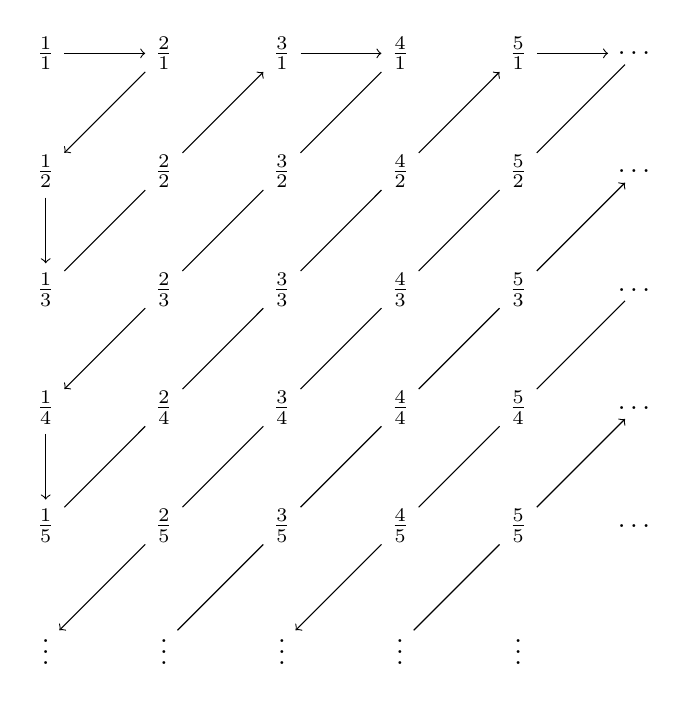
\begin{tikzpicture}
        \foreach \x in {0,...,4}
            \foreach \y in {0,...,4} 
                \pgfmathsetmacro{\numerator}{int(\x+1)}
                \pgfmathsetmacro{\denominator}{int(\y+1)}
                \node (\x\y) at (1.5*\x,-1.5*\y) {$\frac{\numerator}{\denominator}$};

        \foreach \z in {0,...,4}{
            \node (5\z) at (7.5, -1.5*\z) {$\dots$};
            \node (\z5) at (1.5*\z, -7.5) {$\vdots$};
        }

        \draw[->] (01)--(02);
        \draw[->] (03)--(04);

        \foreach \x in {0, 2, 4}{
            \pgfmathsetmacro{\xi}{int(\x+1)}
            \draw[->] (\x0)--(\xi0);
        }

        \draw[->] (10)--(01);
        \draw[->] (02)--(11)--(20);
        \draw[->] (30)--(21)--(12)--(03);
        \draw[->] (04)--(13)--(22)--(31)--(40);
        \draw[->] (50)--(41)--(32)--(23)--(14)--(05);
        \draw[->] (15)--(24)--(33)--(42)--(51);
        \draw[->] (52)--(43)--(34)--(25);
        \draw[->] (35)--(44)--(53);
    \end{tikzpicture}
    \]
\end{example}

Now, the rather shocking part of all of this is that the real numbers actually have a bigger cardinality than the natural numbers. No matter how you try to ``count'' them like the above examples, you will always have a real number left over. I will not be providing a proof of this here, as it will require going over something called the power set.

Another interesting consequence results from the fact that the real numbers consist of rational and irrational numbers. The rationals, though not strictly stated, also have a cardinality of $\aleph_0$ (can you see why?). This implies that what makes the real numbers bigger than the naturals is the irrational numbers, which leads us to realizing that there are many more irrational numbers than rational numbers.

\subsection{Functions in Algebra and Calculus}

In this book, we'll principally be concerned with functions that deal with real numbers. It will be assumed that our functions are all in the form $f : \R \longrightarrow \R$ for our purpose, especially so since we're dealing with single-variable calculus. Here are several examples of them.

\begin{example}
$f(x) = x^2$
\end{example}

\begin{example}
$f(x) = \cos(x)$
\end{example}

\begin{example}
$f(x) = e^x$
\end{example}

It's very obvious to note, but the reason why it's called single-variable calculus is because our functions depend on the single variable $x$ in all of the above functions. 

On the other hand, in multivariable calculus, we deal with functions of the form $f : \R^n \longrightarrow \R^m$. 
\begin{align*}
    f(x_1, x_2, ..., x_n) = (y_1, y_2, ..., y_m)
\end{align*}

We probably won't ever get into these, so you don't really have to worry about them. 

\section{Fractions}

Though frightful to hear, I've unfortunately been alerted by a few people that many college students don't even know how to do simple arithmetic with rational numbers. Here we'll briefly go over the topic.

\subsection{What is a rational number?}

\begin{definition}
A \textit{rational number} is a number that can be represented as a fraction $\frac{p}{q}$ of two integers. $p$ is denoted the numerator of the fraction, while $q$ is denoted the denominator. 
\end{definition}

Just to make it abundantly clear, rational numbers \textbf{are} fractions. It's possible to do arithmetic with them, as you might have already learned in middle school. Here we'll very quickly review and strengthen these concepts. We'll go over multiplication first, since it is much, much easier than addition.

\begin{align*}
    \frac{a}{b} * \frac{c}{d} &= \frac{ac}{bd}
\end{align*}

Here's how to add two rational numbers together. The biggest thing to be careful of is to make sure that the denominators of the two fractions are equal.

\begin{align*}
    \frac{a}{b} + \frac{c}{d} &= \frac{a}{b} * \frac{d}{d} + \frac{c}{d} * \frac{b}{b}\\
    &= \frac{ad}{bd} + \frac{bc}{bd}\\
    &= \frac{ad + bc}{bd}
\end{align*}

It's important to note that division and subtraction is just a special case of multiplication and addition. For example, division is simply equal to the following.
\begin{align*}
    a \div b = a * \frac{1}{b}
\end{align*}
Likewise, subtraction is just a special case of addition.
\begin{align*}
    a - b = a + (-b)
\end{align*}
It is trivial to apply this knowledge to see how division and subtraction works for the rationals. As a matter of fact, fractional division would devolve into the following.

\begin{align*}
    \frac{a}{b} \div \frac{c}{d} &= \frac{a}{b} * \frac{1}{\frac{c}{d}} \\
    &= \frac{a}{b} * \frac{d}{c} \\
    &= \frac{ad}{bc}
\end{align*}

Let's take a look at fractional subtraction. 

\begin{align*}
    \frac{a}{b} - \frac{c}{d} &= \frac{a}{b} + \frac{-c}{d}\\
    &= \frac{a}{b} * \frac{d}{d} + \frac{-c}{d} * \frac{b}{b}\\
    &= \frac{ad}{bd} + \frac{-bc}{bd}\\
    &= \frac{ad - bc}{bd}
\end{align*}

Thus we have characterized the four arithmetic operations in the rationals. Let's move on.

\section{Irrational Numbers}

Irrational numbers are numbers that are simply unable to be represented as a fraction. They can be estimated, sure, but you'll never have a nice, whole representation of what an irrational number looks like on paper. Unless you use symbols like $e$ or $\pi$. But that's kind of cheating. 

This section won't necessarily cover the arithmetic of irrational numbers. We know we can add, multiply irrationals, and that's kind of enough. Instead, this section will try to convince you that irrational numbers are a very real thing (hence why they're a part of the real numbers). 

What does it even mean to be unable to represent a number wholely? You may have heard before that the square root of 2 is an irrational number. Why don't we prove that it actually is?

The following proof follows a strategy known as \textit{reductio ad absurdum}. That is, we take a proposition that we are trying to prove, negate it (take the opposite of that statement), and prove that this negation is impossible. This is also known as a proof by contradiction. 

\begin{theorem}
    $\sqrt{2}$ is irrational.
\end{theorem}
\begin{proof}
    This is a proof by contradiction, so we first negate our proposition and assume that $\sqrt{2}$ is \textbf{not} irrational.

    Now we attempt to show that this is a silly assumption to have. Assume that $\sqrt{2}$ is indeed rational, and can be represented with the \textbf{irreducible} fraction $\frac{a}{b}$. That means the numbers $a$ and $b$ have no common factors. Then,

    \begin{align}
        \sqrt{2}^2 &= 2\\
        \left(\frac{a}{b}\right)^2 &= 2 \\
        \frac{a^2}{b^2} &= 2\\
        a^2 &= 2b^2
    \end{align}

    We see here that $a^2$ is even, and $a$ is even as well as a result. That means $a = 2k$ for some integer $k$. Let's substitute that for (1.4) above.

    \begin{align}
        a^2 &= 2b^2\\
        (2k)^2 &= 2b^2\\
        4k^2 &= 2b^2\\
        2k^2 &= b^2
    \end{align}

    What happened here? We just proved that $b^2$ is also even, and by association $b$ is also even. Thus, we know that both $a$ and $b$ are even numbers... 

    But hold on. Didn't we say in the beginning of this proof that $a$ and $b$ must have no common factors? 

    Aha! A contradiction! Thus, it is impossible that $\sqrt{2}$ can be a rational number, implying that it is irrational instead.
\end{proof}

The beautiful proof above was actually a work of Aristotle. Hopefully it was a good enough proof on the existence of irrationals. 

\section{Notes on Approximation}

In high school and perhaps even a part of college, you were probably taught to \textit{approximate the solution to n significant figures} given a problem. The following is an example and the solution to a problem a student might encounter.

\begin{example}
Compute $\ln(25)$. Round up to 3 significant figures.
\end{example}
\textbf{Solution.}
\begin{align*}
    \ln(25) &= 2\ln(5)\\
            &= 2(1.60943791243...)\\
            &= 3.219
\end{align*}

Approximations are a handy skill to have for the sciences. It's hardly useful for math, however. Approximating an answer gives an inaccurate solution and makes it difficult for both the instructor and the student to check whether or not it is actually correct. In example, the answer $2\ln(5)$ would have been absolutely sufficient as a solution. 

Thus for the rest of the book, we will assume that exercises that come with computations will not require approximations. It is completely fine to leave fractions as fractions, $\pi$ as $\pi$, et cetera. \textbf{Any answers to exercises that get approximated will be marked wrong.}

That being said, if you would like to learn more about scientific approximations to computations, I could write up a short article explaining it. It will detail methods to calculate the accuracy of your approximation, and how this accuracy might blow up when you use the approximation for different calculations.

\section{Practicing Good Mathematics}

This leads us to the final section in this chapter, \textit{practicing good mathematics}. The topic of communicating mathematics is just as important as doing mathematics. After all, what use is there in writing incoherent solutions to problems if no one can verify your work? Here we will explore some of the skills you may want to pick up when writing down your work.

\subsection{Consider your audience}

The age-old concept for writing essays applies just as well for writing mathematics. When you write a solution, a proof, or even an explanation of a concept, \textit{consider who you are writing for}. Are you writing this for your instructor? A fellow student? Yourself? Depending on who your audience is, your work might get maximally confusing for some. 

Consider this book for example. I am writing this book with a very specific person in mind as my audience. As a result, I want the content of this book to be digestible for a person who hasn't had the traditional education of mathematics. It should be easy to follow, and easy to read. Hopefully I'm doing a pretty good job at that. Let me know otherwise.

On that note, it might help to specify a specific \textit{person} as your audience when you're writing. In your case, this shouldn't be too difficult-- you're writing to me, the author. When you're writing solutions, consider the type of writing I might appreciate. Try not to get too wordy. Don't throw around meaningless symbols without explaining what they do. You don't have to explain elementary concepts to me from scratch, since I (hopefully) should know them already. Keep this in mind as you write, and you'll be fine.

\subsection{Explain what you're doing}

This is traditionally what a teacher means when they tell you to show your work. It gets impossibly difficult to tell whether or not you actually understood the material if you don't show your steps properly. 

Here are two solutions to an elementary derivation problem. Hopefully you can tell which one is a better solution even without understanding how the work was done. 

In the below example, the notation $\frac{df}{dx}$ and $f'(x)$ notates the derivative of the function $f$ with regards to the variable $x$. If you don't really know what that means, don't worry about it.

\begin{example}
Compute $\frac{df}{dx}$ given $f(x) = \frac{6x^2}{2-x}$.
\end{example}

\textbf{Solution 1.}
\begin{align*}
    f'(x) = \frac{6x(4-x)}{(2-x)^2}
\end{align*}

\textbf{Solution 2.}
\begin{align*}
    f'(x) &= \frac{d}{dx}\left(\frac{6x^2}{2-x}\right)\\
        &= \frac{(2-x)\frac{d}{dx}(6x^2) - 6x^2\frac{d}{dx}(2-x)}{(2-x)^2} \text{ (quotient rule)}\\
        &= \frac{(2-x)(12x) - 6x^2(-1)}{(2-x)^2}\\
        &= \frac{(24x-12x^2) + 6x^2}{(2-x)^2}\\
        &= \frac{24x-6x^2}{(2-x)^2}\\
        &= \frac{6x(4-x)}{(2-x)^2}\\
\end{align*}

That being said, keep in mind that you're writing to me. You don't have to precisely explain every single thing you're doing to solve a problem. 

\subsection{Draft your work}

It's a known fact that a first draft of anything is going to be a mess. Therefore, it's best that you keep a sheet for scratch work, and another sheet for writing down answers. 

Keep your work organized, but don't try to write up a good answer from the get-go! Keep your first draft organized enough so that you can follow your work and refer back to it if needed.

\subsection{References}

This subsection took some references from Francis Su's \cite{su:2015} article on good mathematics. It also references Paul Halmos' \cite{halmos} essay on good writing, though I suspect this is much less useful for you than for me. 

\section{Exercises}

\begin{exercise}{1.5.1}
Find the domain and range of $f(x) = \cos(x)$. Do the same for $g(x) = \tan(x)$. It will help for you to remember that $\tan(x) = \frac{\sin(x)}{\cos{x}}$. If you do not remember what trigonometric functions look like, you may use the graph to help you out. 
\end{exercise}

\begin{exercise}{1.5.2}
Find the domain and range of $f(x) = x^2$.
\end{exercise}

\begin{exercise}
Find the domain and range of $f(x) = 1$.
\end{exercise}

\begin{exercise}
Consider the function $x^2 + y^2 = 25$. Is this a valid function? Why or why not?
\end{exercise}

\begin{exercise}
Consider the function $f(x) = \pm\sqrt{x}$. Is this a valid function? Why or why not? 
\end{exercise}

\begin{exercise}
Compute $\frac{3}{7} + \frac{5}{11}$.
\end{exercise}

\begin{exercise}
Compute $\frac{3}{96} + \frac{9}{36}$. 
\end{exercise}

\begin{exercise}
Compute $\frac{3}{7} * \frac{5}{11}$. 
\end{exercise}

\begin{exercise}
\textbf{Challenge.}
Simplify $\frac{1}{(x+1)} + \frac{1}{(x-1)}$. 
\end{exercise}

\begin{exercise}
\textbf{Challenge.}
Consider a function $f : \Q \longrightarrow \Z$ (recall $\Q$ is the set of rationals), where $f(\frac{p}{q}) = p * q$. Explain why $f$ is not a valid function. \textit{Hint: Notice that $\frac{1}{2} = \frac{2}{4} = \dots$}
\end{exercise}

\chapter{The Algebras}
\epigraph{A lot of times, when kids have problems with algebra or trigonometry, it has nothing to do with the subject matter, has nothing to do with their innate intelligence. It's just they that they had some gaps in elementary school that they never got to fill in.}{Sal Khan}

Why do we care about Algebra? Perhaps the question isn't too difficult for you, given your accounting background. Algebra is the backbone of mathematics, and it's what gets used to solve countless numerical problems that require logic. Any time you need to know the solution of an equation, or when you need to consider the behaviors and the quantities of these solutions, Algebra is what gets used to uncover these mysteries. 

So in this chapter, we'll explore some of the ways this beautiful subject gets used in real life. Hopefully the examples will be able to motivate your studies as an accountant.

\section{Systems of Equations}

What would a person do if they needed to find a common solution to a series of interconnected relationships? If the set of relationships mentioned happened to be a series of linear equations (which it very often is), then we have something called a \textit{System of Linear Equations}. Here we go over how to find the solutions to such problems. 

\subsection{Introduction to System of Linear Equations}

Before we go anywhere with this idea, we must first discuss what a linear equation even is. You might remember from oh-so-long-ago that a linear equation might be a simple equation for a line. In the two-dimensional case where we just deal with x and y, this is true. But if we extend out to the third dimension, we see that an equation of a plane is a linear equation as well.

So what is a linear equation, then?

\begin{definition}
  A \textit{linear equation} is an equation that may be put in the form 
  \begin{align*}
    a_0x_0 + a_1x_1 + \dots + a_nx_n + b = 0
  \end{align*}
  where the $a_i$ and $b$ are real constants, and $x_i$ are variables.
\end{definition}

Below are some examples of linear equations. Notice how the first three of the examples are all actually the same equations in different forms.

\begin{example}
  \begin{enumerate}
    \item $y = 2(x + 5)$
    \item $y - 2x = 10$
    \item $y -2x -10 = 0$
    \item $x + 5 = 0$
    \item $x + y + z = 0$
    \item $2x_0 + 3x_1 + 4x_2 + 5 = 0$
    \item $x + z = 10$
    \item $10x_0 + x_3 = 2$
  \end{enumerate}
\end{example}

A system of linear equations is when there are more than one of such linear equations in a set. Below is an example of such a system.

\begin{example}
  \[
    \begin{cases}
      x + y = 2\\
      2x + 3y = 5
    \end{cases}
  \]
\end{example}

A principal interest concerning these systems of equations is to find a common solution satisfying all of these linear equations. For example, the solution to the above system would be the pair $x = 1, y = 1$. 

It's essential to note here that you don't always have a unique solution like we did here for a system of equations. As a matter of fact, it's a pretty special thing for a system of equations to have a unique solution. Here are two trivial systems where one has no solutions, and the other has infinitely many solutions. Can you see which is which?

\begin{example}
  \[
    \begin{cases}
      x + y = 0\\
      x + y = 0
    \end{cases}
  \]
\end{example}

\begin{example}
  \[
    \begin{cases}
      x + y = 0\\
      x + y = 5
    \end{cases}
  \]
\end{example}

It would be nice if there was an algorithm we could work through in order to always find the solution(s) to any given system of equations. Well, you'll be elated to learn that our mathematicians have been very hard at work, and managed to come up with an algorithm just in time. But before we get there, we'll need to build some intuition by exploring different methods of finding the solutions to linear equations. 

\subsection{Solving by Graphing}

Barring the odd stuff like abstract and futurist art, it's often visual beauty that speaks out to us most vividly. Things aren't so different in mathematics. It's the visual proofs that makes the most intuitive sense to us. So, we shall start off our solution-finding journey from a geometric viewpoint.

So long as we are working in up to three variables, we can graph any equation. Given one variable, we just plot a point in a line. Given two variables, we graph a line on a plane. Given three variables, we draw a plane in a 3-dimensional space. Given four variables... well, we don't have a way of graphing that visually. 

So given a system of equations, we'll do the most obvious thing and graph all of the equations. Each graph of an equation will represent the set of solutions to that specific equation. Then, finding the solution to our system is as simple as finding the point where all our equations intersect. Let's consider the following system.

\begin{example}
  \[
    \begin{cases}
      x + 4y = 2\\
      2x + 3y = 5
    \end{cases}
  \]
\end{example}

Below, the graph drawn in blue will represent the equation $2x + 3y = 5$. The graph in red is $x + 4y = 2$. 

\begin{figure}[H]
  \includegraphics[width=7cm]{system-of-eqs.png}
  \centering
  \caption{Graph of a system of equations}
\end{figure}

We can see that there exists a solution where $x=2.8$ and $y = -0.2$. Okay, let's try that again with 3 equations this time. 

\begin{example}
  \[
    \begin{cases}
      x + 4y = 2\\
      2x + 3y = 5\\
      2x + 3y = 4
    \end{cases}
  \]
\end{example}

\begin{figure}[H]
  \includegraphics[width=7cm]{system-of-eqs(2).png}
  \centering
  \caption{Graph of a system of equations}
\end{figure}

Uh-oh. Now there's a problem. There's no common point of intersection! This indicates that the 3-equation system has \textit{no solutions}.

This is a pretty intuitive way of looking at systems of equations and their solutions. But the geometry falls apart pretty quickly once we start using four or more variables. At that point, we need to pull out the big guns: algebra. 

\subsection{Solving Through Elimination}

Recall that an equation is a statement asserting the \textbf{equality} of two equations. Thus our new method will very obviously have to take advantage of one of the properties of equality. Consider the following property. 

\begin{center}
  Given a, b, and c, if $a = b$, then $a + c = b + c$. If $c = d$, then $a + c = b + d$. 
\end{center}

We can apply this to our system of equations. Let's take a look at the system below. 

\begin{example}
  \[
    \begin{cases}
      x + 4y = 2\\
      2x + 3y = 5
    \end{cases}
  \]
\end{example}

Let $a = 2x + 3x$, and $b = 5$. Then $c = x + 4y$ and $d = 2$. Then, our $a + c = b + d$ would be 

\begin{align*}
  3x + 7y = 7
\end{align*}

This is not very useful for our purpose. But what if we look at $a - c = b - d$?

\begin{align*}
  x - y = 3
\end{align*}

We can apply the process one more time to look at $a - 2c = b - 2d$. 

\begin{align*}
  - 5y = 1
\end{align*}

Then, with a little bit of algebraic manipulation, we see that $y = -\frac{1}{5}$. Substituting this value into $x + 4y = 2$, we see that $x - \frac{4}{5} = 2$ and $x = 2 + \frac{4}{5} = 2.8$. 

\textbf{tl;dr} So, going back to our initial system, we essentially took the first equation and subtracted it twice from the second equation in order to \textbf{eliminate} the $x$ variable. Of course, this process can be used to eliminate any variable(s) from an equation in a system. 

\subsection{Word Problems}



Let's start off with an example that I found from 1994 by a writer called Eisner \cite{eisner:1994}.

Say Steve and Jacob held stock in a corporation at a ratio of 75 percent to 25 percent. Steve's stock was worth \$19500, while Jacob's stock was worth \$6500. 

\subsection{Problems}

\section{Polynomial Arithmetic}

Here we will cover polynomial multiplication, factorization, and division.

\section{Polynomial Factoring}

\subsection{Problems}

\section{Rational Exponents}

\section{Exponentials and Logarithms}

\subsection{Problems}

\section{Trigonometry}

\subsection{Problems}

\printbibliography

\end{document}
